\section{Introduction}

Image annotations are required in a wide range of applications
including image classification (which requires textual labels),
object detection (bounding boxes), or image segmentation (pixel-wise classification).
The rise and successes of deep learning lead to an increasing need for annotations,
as training sets should be of a large size for these algorithms to be efficient.
Yet, researchers still spend time and resources
to create ad hoc tools to prepare those datasets.
The application we present in this paper aims at providing a customizable tool
to fulfill most image annotation needs.

\begin{table*}[ht]

\begin{tabular}{lclllcc}
Application
	& Year
    & Tools
    & \makecell[l]{Configurable\\interface}
    & \makecell[l]{Tasks\\management}
    & Type
    & License \\
    \midrule
LabelMe
	& 2008
    & bbox, polygon, iterative semi-automatic segmentation
    & no
    & Mturk integration
    & server
    & OSS \\
VIA
	& 2016
    & bbox, polygon, point, circle, ellipse
    & no
    & no
    & client
    & OSS \\
Labelbox
	& 2018
    & bbox, polygon, point, line
    & yes
    & yes
    & server
    & private \\
Dataturks
	& 2018
    & bbox, polygon
    & no
    & yes
    & server
    & private \\
Ours
	& 2018
    & bbox, polygon, point, stroke, outline
    & yes
    & Mturk integration
    & client
    & OSS \\
\end{tabular}

\caption{Most relevant image annotation Web applications.}%
\label{tab:web-apps}
\end{table*}

% \begin{figure*}[ht]
%     \centering
%     \begin{subfigure}[b]{0.575\textwidth}
%         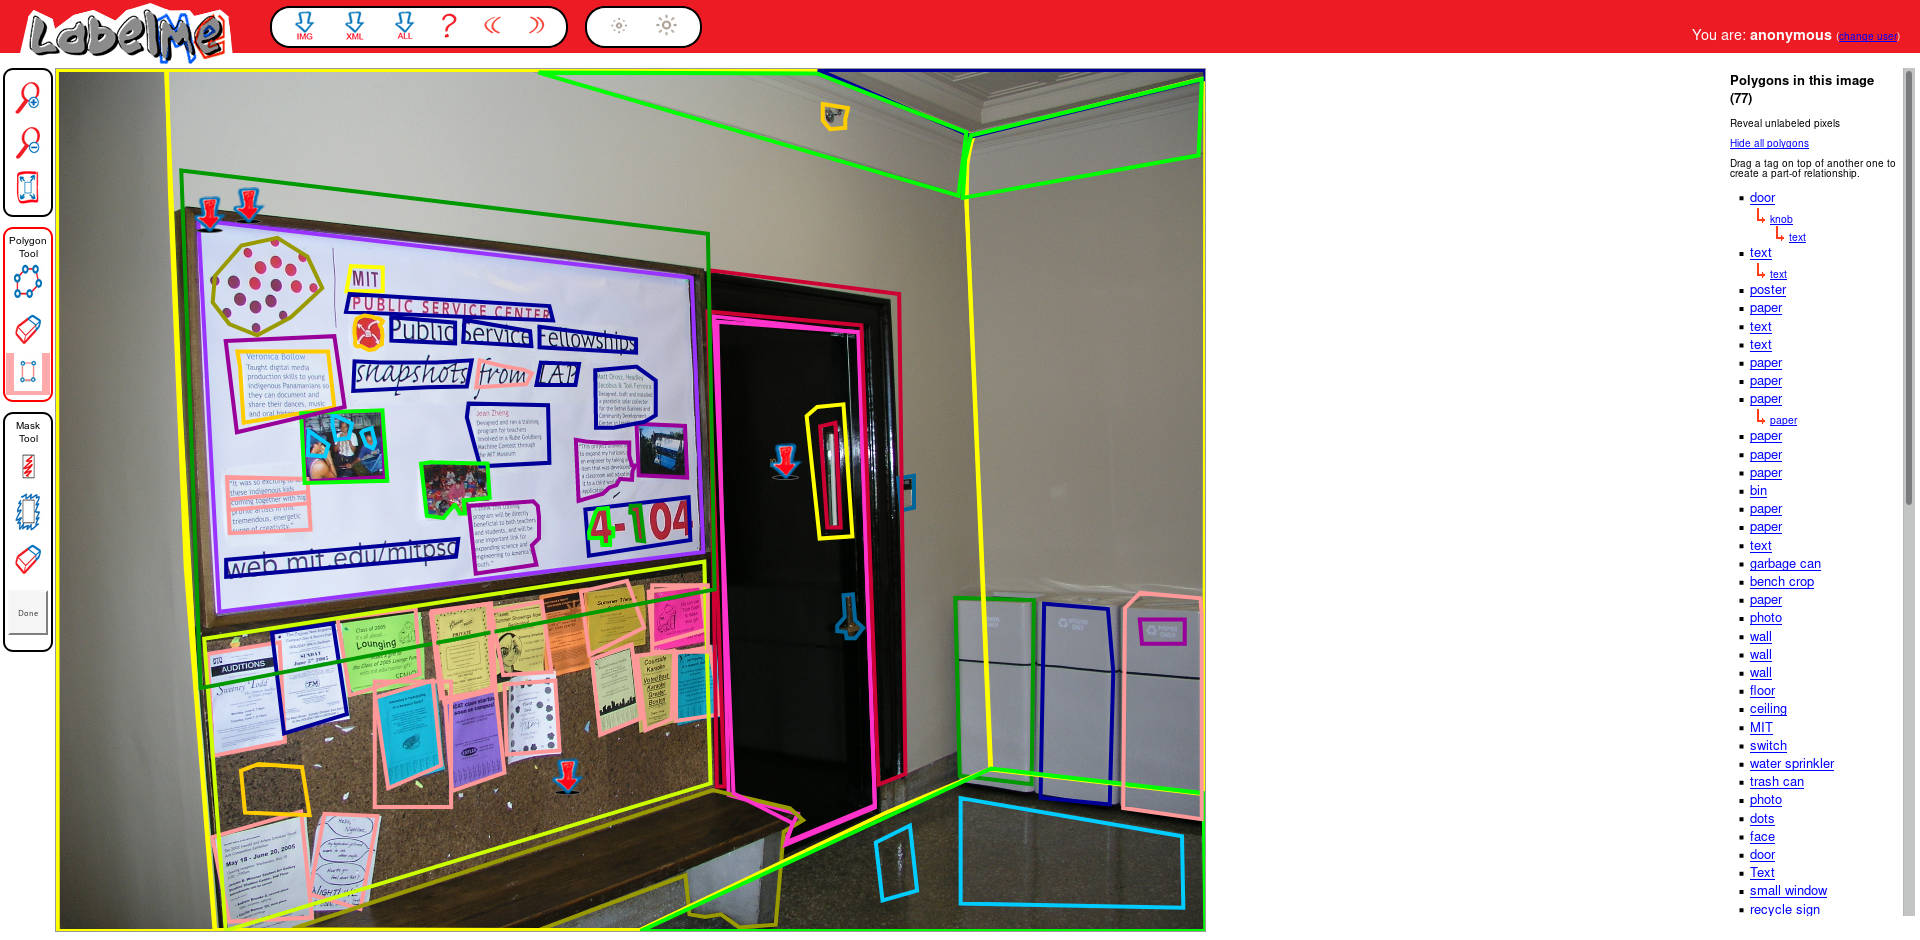
\includegraphics[width=\textwidth]{img/labelme.jpg}
%         \caption{LabelMe}
%     \end{subfigure}
%     \hfill
%     \begin{subfigure}[b]{0.405\textwidth}
%         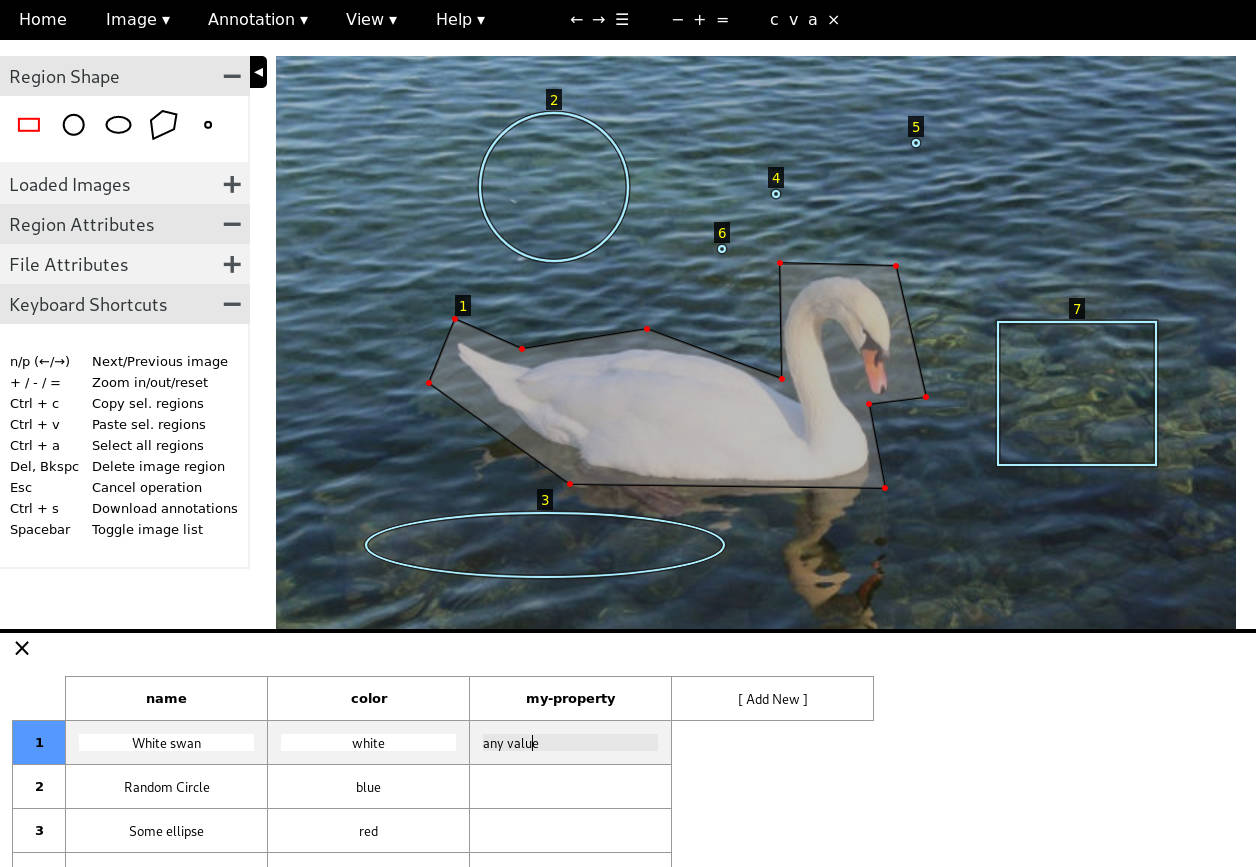
\includegraphics[width=\textwidth]{img/via.jpg}
%         \caption{VIA}
%     \end{subfigure}
%     \hfill
%     \begin{subfigure}[b]{0.42\textwidth}
%         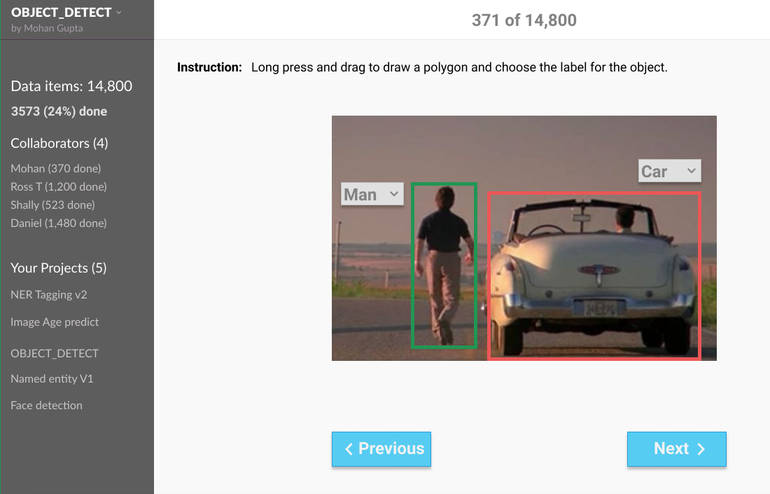
\includegraphics[width=\textwidth]{img/dataturks.jpg}
%         \caption{Dataturks}
%     \end{subfigure}
%     \hfill
%     \begin{subfigure}[b]{0.56\textwidth}
%         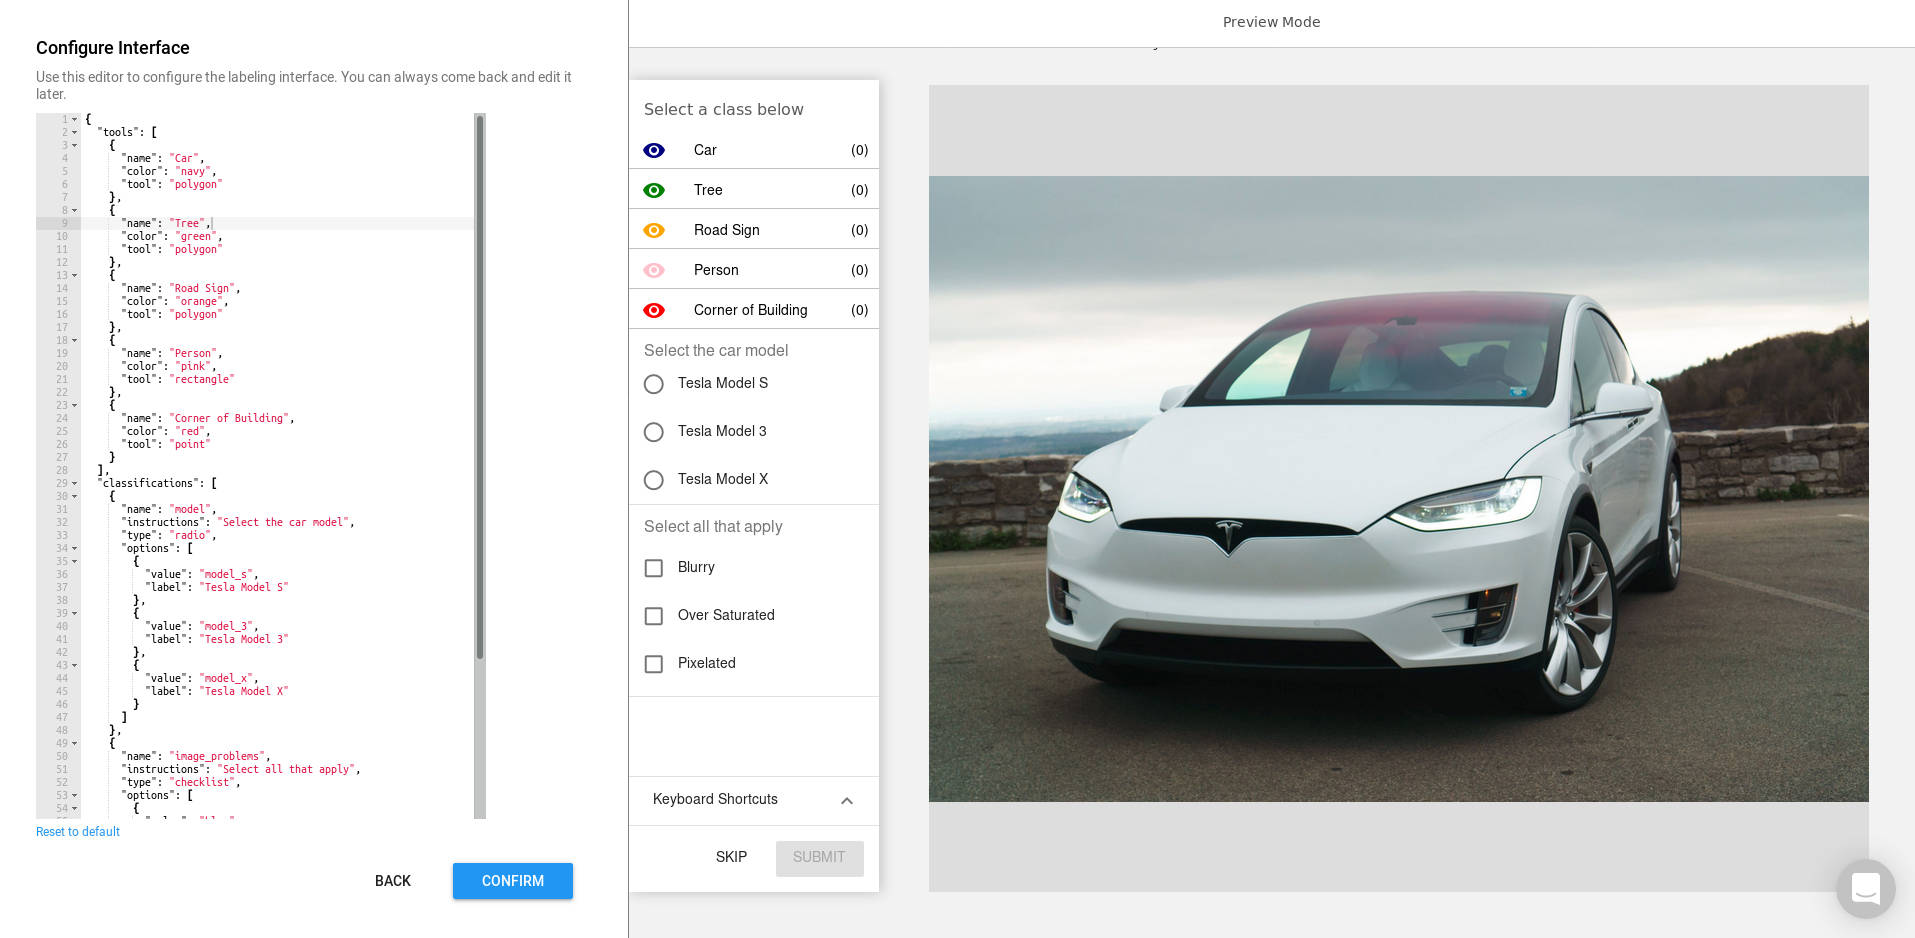
\includegraphics[width=\textwidth]{img/label-box-config.jpg}
%         \caption{Labelbox}
%     \end{subfigure}
%     \caption{Interfaces of main other Web annotation applications}\label{fig:interfaces}
% \end{figure*}

Many image annotation applications already exist (Table~\ref{tab:web-apps}).
LabelMe~\cite{russell2008labelme}, one of the most popular,
provides an interface for drawing bounding boxes and polygons
around objects in an image.
It has been used extensively to create datasets for image segmentation.
Some more recent softwares share the same goals, with their own specificities.
For example, Labelbox~\cite{labelbox} and
Dataturks~\cite{dataturks} provide annotation tasks management,
particularly useful when crowdsourcing the annotations;
these softwares are proprietary.
The VGG Image Annotator (VIA~\cite{dutta2016via})
is an open-source client application like ours,
with the specificity of providing annotation attributes,
editable in a spreadsheet format.

We release an open-source application~\cite{annotationappgithub},
entirely client side, meaning that no data is uploaded to any server.
Images are loaded from files and annotated locally, in the browser.
The simplest tool, from a user perspective, should be immediately available
i.e.\ should not require any additional installation to be fully functional.
Our image annotation software is thus a Web-based application,
easily configurable to fit users needs, as well as
embeddable in the Mechanical Turk platform to design crowdsourcing campaigns.

We first present the features of our application, then describe its architecture.
Finally, we explain how it can be used to start crowdsourcing experiments.
